% \section{Motivation}
\section{Problem Setup}
% \todo{rename throughput profiles -> bandwidth profiles}
%Overlay multicast in the cloud presents a number of new considerations, such as cloud pricing models for networking and compute resources as well as resource constraints (e.g., instance limits, per-VM egress limits) imposed by providers.

We frame the problem of cloud multicast in terms of constructing an overlay network for replicating data, which involves defining:
% 
(1) the set of \textit{overlay nodes} (i.e., cloud VMs) and (2) the \textit{paths} between those nodes that will be included in a multicast replication tree.
% 
\sys eventually divides the target data into multiple \textit{stripes} (i.e., partitions), so concurrent replication trees may be used in a single transfer.
%\sarah{I wonder if we should move this to the intro, or if its too much detail?}
%VL: See note in intro
Our optimization objective is to minimize the monetary cost of replication while also meeting a replication time constraint.
%
%The time constraint is critical as many applications require a Service Level Objective (SLO) on the transfer completion time.
% 
%For example, disaster recovery requirements may aim to copy data to multiple clouds within a bounded time to minimize data unavailability upon an outage.
% 
%As a reference point, AWS Replication Time Control offers a 15-minute transfer completion time SLO~\cite{aws-replication-time-control}.
%
%VL: below is redundant
%Multicasting data with sufficient throughput and minimal cost requires balancing these two concerns using
% the above knobs, i.e., 
%the number and location of overlay nodes and paths.
%we must select the number and location of overlay nodes and the paths that data is replicated to achieve the right balance between replication cost and throughput.

% In the remainder of this section, we describe the characteristics of the cloud that are relevant for cost-optimizing cloud multicast. 

% The cost-optimized cloud multicast problem is fundamentally different from the classic network multicast problem:
% \begin{enumerate}
%     \item Variable egress pricing by source and destination
%     \item Variable network bandwidth by source and destination
%     \item Elasticity to mitigate source-region egress limits
% \end{enumerate}

% We explain each difference in isolation then illustrate the full problem space with a simple example.

\begin{figure}[tbp]
     \centering
     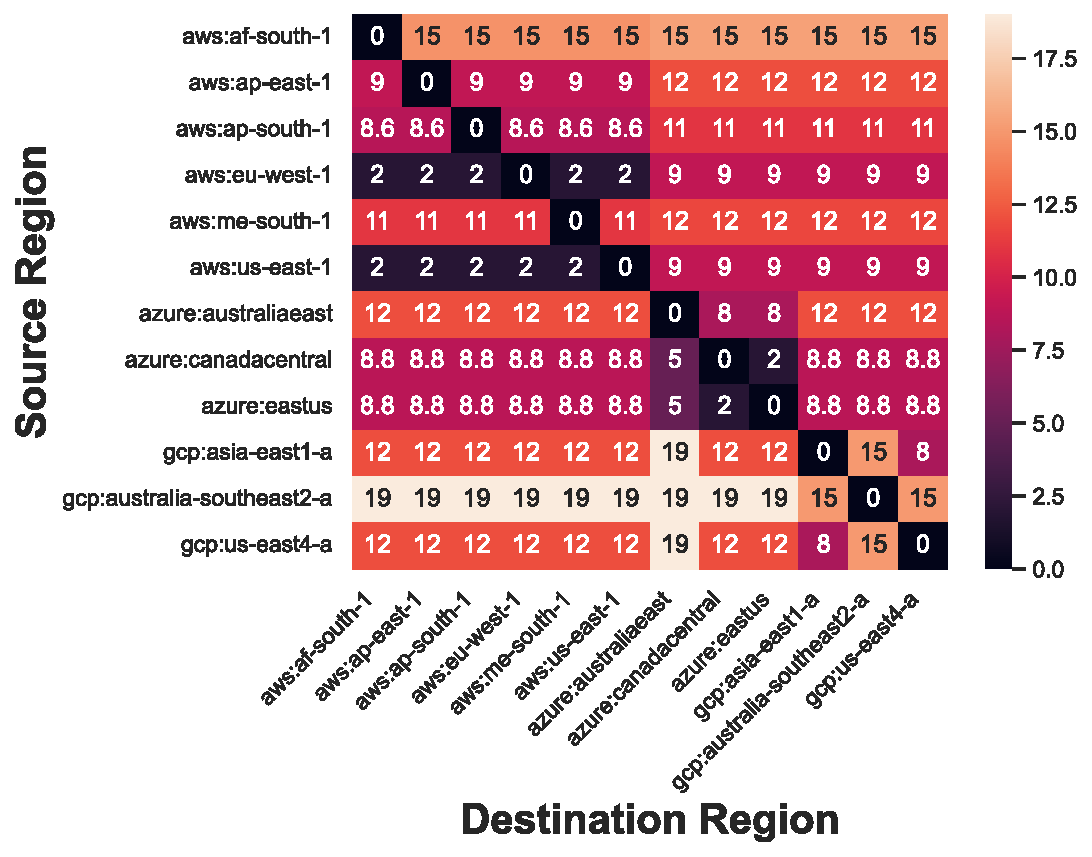
\includegraphics[width=0.9\linewidth]{figures/cost_heatmap.pdf}
     %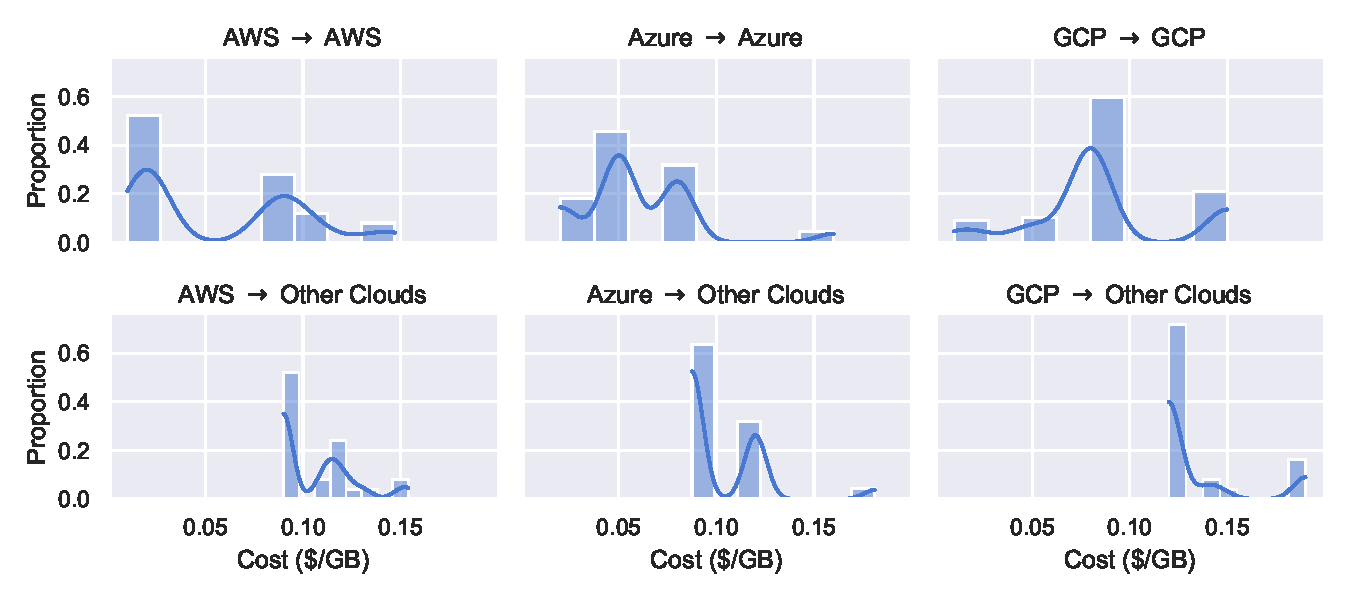
\includegraphics[width=\linewidth]{figures/2-3-cost-histograms.pdf}
     \caption{Egress fees between regions (in cents per GB).}
     \label{fig:cost_heatmap}
\end{figure}
% \sarah{explain setup of we want to transfer data across regions - and then explain how we can use VMs to transfer data, and now we want to decide on that overlay structure}
\subsection{Egress Costs}
A unique aspect of multicast in the cloud is the effect of egress costs incurred for data transferred across cloud regions.
%
Cloud providers charge for wide-area data transfer \textit{per-GB} of data transferred.
% 
Egress prices---as a method of keeping data within the provider's regions without disincentivizing migration into the provider---dominate data movement costs in the cloud and fundamentally change the multicast problem.
% \vincent{how? give some intuition}\joey{I think this is addressed in the figure but we could/should do better for the camera ready.}
% 
Figure \ref{fig:cost_heatmap} visualizes the pricing for 11 regions across AWS, Azure, and GCP.
% 
Prices vary depending on the source and destination cloud or region, with differences of up to $23\times$ across region pairs.
%
Along those lines, one particularly important axis is whether the transfer stays within a given cloud provider or crosses provider boundaries, as inter-cloud egress costs are generally higher than intra-cloud egress.



Intra-cloud egress (data movement between geographically separated datacenters in the same cloud provider)
% , at the time of writing, 
is priced between $\$0.01-\$0.19$ per GB transferred.
% 
Prices typically increase with longer-distance transfers.
% 
For example, GCP charges $\$0.08$ for transfers between continents but only $\$0.02$ for transfers within the US.
% 
Some smaller providers (e.g., IBM, Cloudflare) offer free cross-region egress.

Inter-cloud egress (data movement between different cloud providers) is typically priced at a much higher rate per GB ($\$0.08-\$0.23$).
% 
As such, it is essential to minimize cross-cloud transfers in a multicast replication tree.

\begin{figure}[tbp]
     \centering
     % 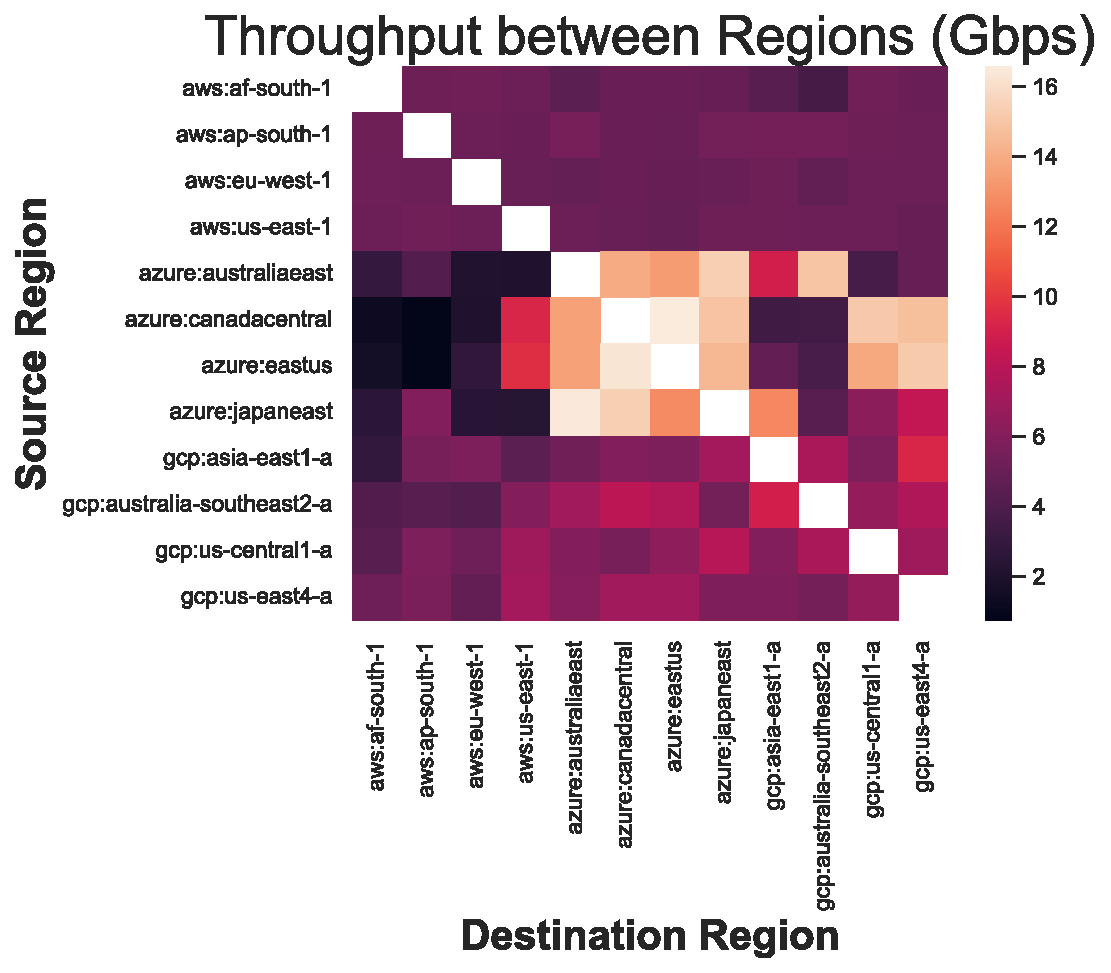
\includegraphics[width=\linewidth]{figures/tp_heatmap.pdf}
     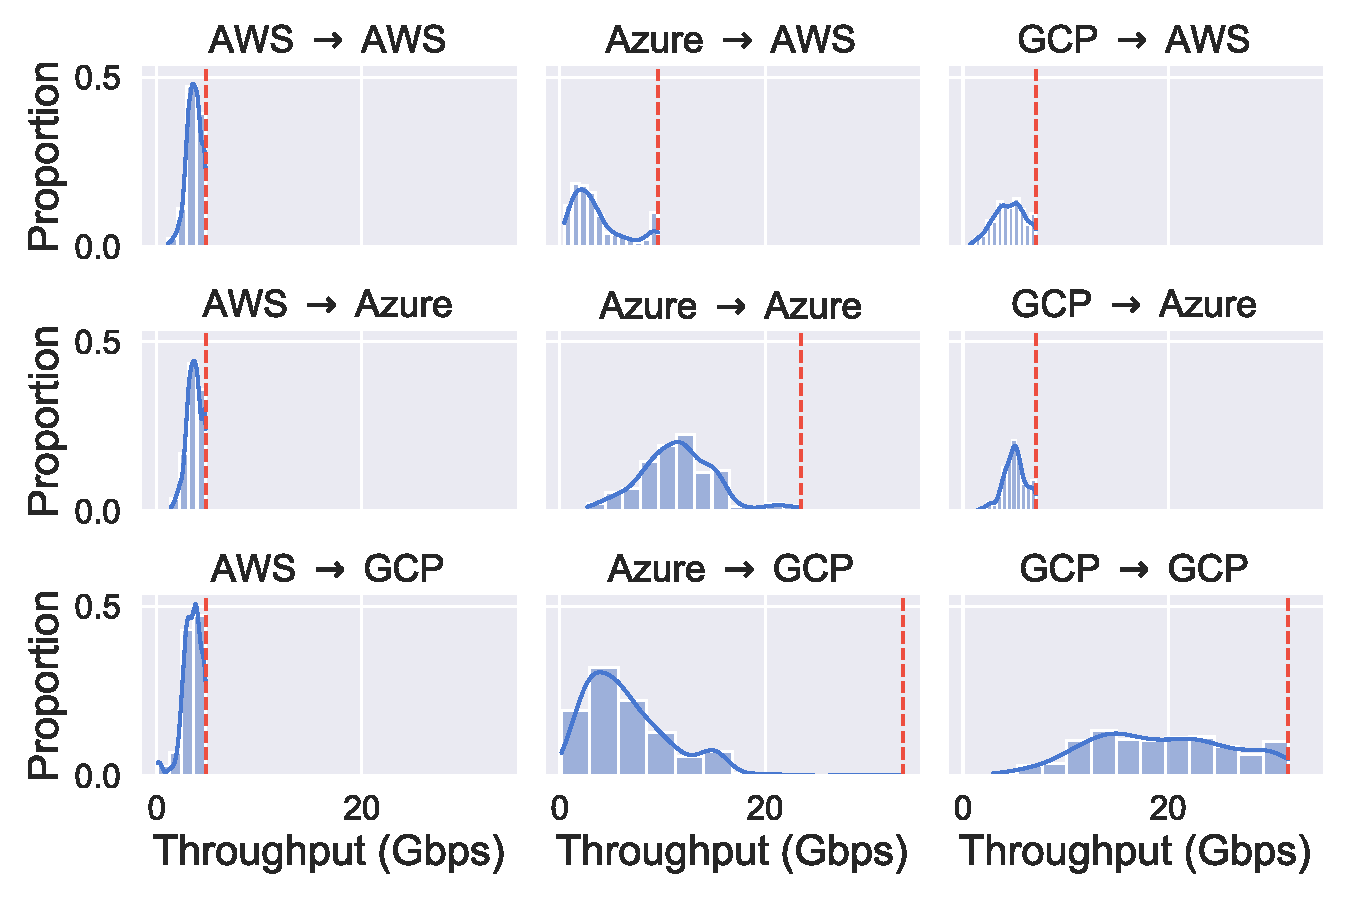
\includegraphics[width=0.9\linewidth]{figures/3-3-throughput-histograms-no-share-x.pdf}
     \caption{Bandwidth distribution (in Gbps) between regions. Per-VM egress limits are marked in red dotted lines.} %Bandwidth varies significantly across regions and providers. 
     %AWS limits cross-region egress to 5\,Gbps, so have lower throughput generally. 
     %Azure has high intra-cloud performance but poor performance in the AWS region, except for AWS US East 1.  
     % \todo{Align X-axis to show variation between providers} 
     % \shu{Also the x and y title here is too small} \paras{Show the throughput wall with markings to show infeasible region.}
     \label{fig:tp_hist}
\end{figure}

\subsection{Bandwidth Variability Across Endpoints}
\label{ss:bandwidth-variability}
Meeting replication time constraints can be challenging due to network bandwidth variability in the cloud.
One type of variability arises from cloud providers, who impose constraints on per-VM egress and ingress bandwidth.
These constraints differ significantly across providers:
for instance, AWS throttles intra-cloud and inter-cloud egress to 5\,Gbps per VM, while Azure imposes no VM-level limits.
The impact of these egress limits can be observed in Figure \ref{fig:tp_hist}, where bandwidth is capped at the VM egress limit for AWS and GCP.
Limited node egress poses a particular challenge for cloud multicast, as the source node's egress bandwidth is often the bottleneck.

Even when source-node bandwidth is not the bottleneck, observed network capacity can also vary considerably across cloud region pairs (up to $202\times$).
%
Note that these networks are relatively stable across time; prior work~\cite{jain2022skyplane} has found that network throughputs are stable over periods of at least 24 hours.
%
Instead, variations are primarily observed across different source and destination regions.
% 
Figure \ref{fig:tp_hist} depicts the distribution of profiled bandwidth between VMs running in AWS, Azure, and GCP.
% \joey{how many pairs and for how long?}
% 
Intra-cloud bandwidth is typically (but not always) higher than inter-cloud bandwidth.
%, as each category has significant variability. 

%Meeting replication deadlines can therefore require carefully choosing the replication tree to both leverage high-bandwidth paths across regions and alleviate the effects of source region bottlenecks.

% However, achieving high throughput for replication can be challenging: First, cloud providers control their network traffic to allocate certain amounts of bandwidth to paths between specific regions, limiting the per-VM throughput between regions. \sarah{there should be a better way to say this} Second, cloud providers also impose artifical limits on the network egress and ingress per-VM. 
% For example, AWS limits cross-region egress to 5Gbps per VM, as shown in \cref{fig:tp_hist}. 

% nb paras: this is a soluton space concern
% Meeting these constraints requires selecting the right waypoint regions, number of VMs, and distribution trees for data. To do so, we must optimize both the number of VMs per-region (the overlay node set) and the distribution trees together.  \sarah{Say something about how this increases the search space?} \simon{addressed in previous paragraph, the latency target is about the constriant right?}

\begin{figure*}[tbp]
    \centering
    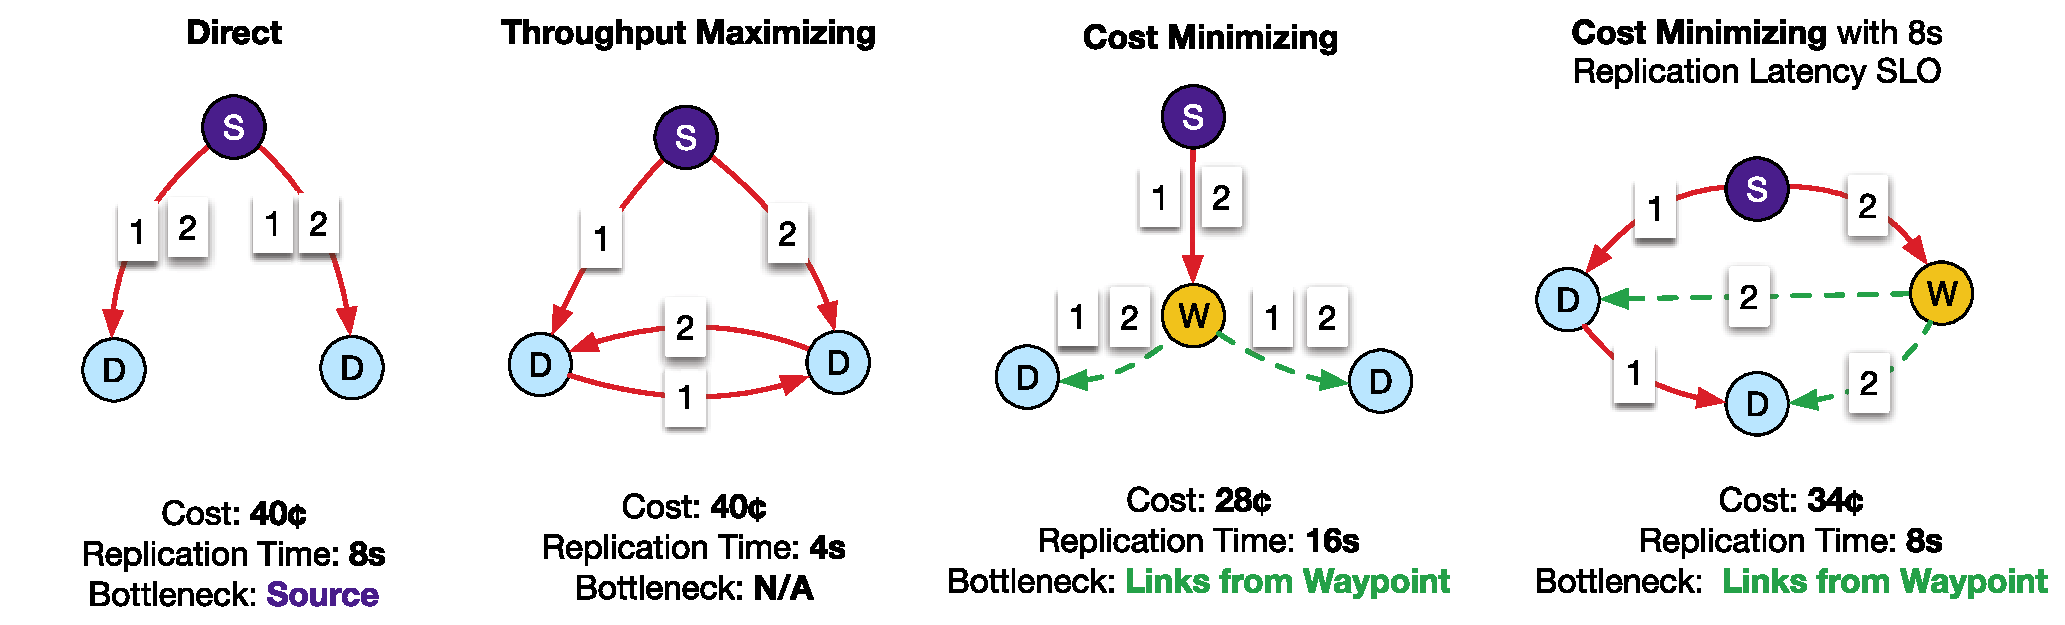
\includegraphics[width=0.9\linewidth]{figures/toy_example.pdf}
    \caption{Overlay node set and distribution trees for a toy example.  The source and destination nodes are marked `S' and `D' respectively, while waypoint nodes in yellow are marked `W'. Expensive, fast paths ($\$0.1$ per GB, $2$\,Gbps) are shown in solid red, while slow, cheap paths ($\$0.02$ per GB, $1$\,Gbps) are shown in dashed green. 
    %In the \textit{Direct} tree, the source node egress (4Gbps) is the bottleneck in sending out 8GB ($4 \times 2$GB stripes) of data, while both the \textit{Cost Minimizing} trees, the outgoing links from the waypoints ($1$\,Gbps) are the bottleneck. For the \textit{Throughput Maximizing} tree, all link bandwidth is used to full capacity (2Gbps) to each send $2$GB stripes, and are not bottlenecked by node egress or other links' bandwidth. 
    \paras{Shouldn't cloudcast be something between 4 and 8s?}
    %\simon{This needs to be move up to earlier pages. This is a good "motivation plot".\sarah{from shu/ion:I got some feedback for the toy example 1) make it more clear on the data size (i.e. putting maybe a small graph right next to those examples showing partition 1/2 aggregate size) and 2) make it more clear on how the replication time is calculated (it’s described in the text and caption, it’s better to have text right next to the link showing what’s the bottleneck bandwidth or something similar to that; make it more intuitive on understanding why the topology is slow)}}
    } 
    \label{fig:toy_example}
\end{figure*}
\subsection{Elasticity of Resources}

%In the multicast setting, source region bandwidth is often a bottleneck.\sarah{this doesn't fit together with the title of the section - need a transition} 
% 
%Prior work like Splitstream~\cite{castro2003splitstream} note this bottleneck with proposed solutions in non-cloud environments.
% 
A major advantage of the cloud is resource elasticity and the ability to flexibly provision VMs across many regions. 
% 
In the face of the source bottlenecks described above, VM elasticity translates to a corresponding \emph{elasticity of bandwidth}.
%
% In other words, 
Allocating multiple parallel VMs enables users to scale throughput beyond per-VM network bandwidth limits.
%
% This is notionally similar to prior work in peer-to-peer overlays (e.g., Splitstream~\cite{castro2003splitstream}) that leverage sharding for performance. \sarah{I dont understand what this means. weren't we jsut using this to reference evidence for source bottlenecks?}\joey{I think the above statement is risky since it relates but doesn't contrast... maybe we comment it out for now?}

%These VMs can be deployed at the source region to directly reduce the impact of source region bottlenecks, which are common in the multicast-setting: for example, prior work like Splitstream~\cite{castro2003splitstream} note this bottleneck with proposed solutions in non-cloud environments.

Unfortunately, adding elastic VM capacity at the source region has limitations.
% 
Additional VMs add additional costs due to per-second billing on VMs, which can impact the cost/throughput tradeoff.
% 
We note that because the marginal cost of additional VMs is often relatively small compared to egress fees, the tradeoff is often worth making.
%it is often possible to significantly increase throughput at only a small marginal increase in cost --- in the cloud, fast can be cheap.
% 
However even in these situations, bandwidth elasticity has limits: for instance, if a network-based bottleneck is unavoidable or when cloud providers limit the number of vCPUs per region. 

%\sarah{maybe better to start with this?} 
Crucially, elastic VM capacity can also be deployed at \textit{waypoint regions} that are neither the source nor the destination.
% 
These waypoint regions can help mitigate source VM bottlenecks by distributing load from multicast fan-out across multiple separate regions.
% 
Waypoint regions also mitigate 
% intermediate 
points of congestion 
% in a transfer 
by routing data around slow paths.
\subsection{Illustrated Example}
Selecting overlay nodes and replication trees to optimize cost and throughput is challenging.
Consider the toy example in Figure \ref{fig:toy_example} for a 2\,GB replication with two 1\,GB stripes.
Assuming a 4\,Gbps bandwidth limit for all nodes and one VM per region, the source (``S'') and destination (``D'') nodes have fast but expensive outgoing paths, capable of sending at 2\,Gbps but costing $10\mbox{\textcent}$ per GB transferred.
Other regions have cheaper but slower outgoing paths, capable of sending at 1\,Gbps but costing $2\mbox{\textcent}$ per GB transferred.
In a simple direct replication scenario, the replication will be bottlenecked by the source node's egress limit (4\,Gbps). With two copies of data to send, the total transfer time will be 8 seconds.

Like many bandwidth-optimized techniques \cite{castro2003splitstream, ganguly2005fast,kostic2003bullet}, we offload egress bandwidth by sending a single data copy from the source and leveraging multiple replication trees. Replication cost is reduced by replicating to a waypoint, and then multicasting to destinations. This doubles replication time to 16 seconds due to stripes being replicated via the slower path (dotted arrows). An 8-second replication SLO is met by transferring just one stripe via the cheaper waypoint.

This simple example presents a large search space for possible replication trees, and real-world cloud networks present additional parameters such as choosing the number of VMs per region and many possible waypoint regions.
